\vfill
\begin{figure}[H]
    \centering
    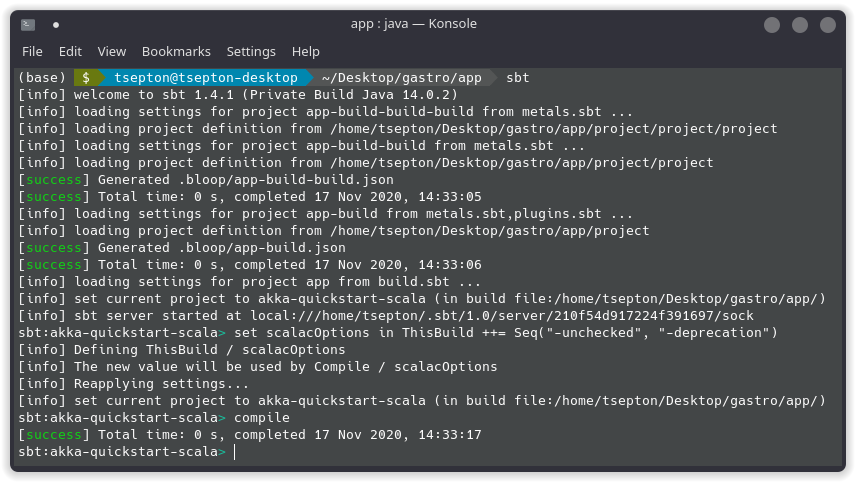
\includegraphics[width=1\textwidth]{parts/pics/1.png}
    \caption{La compilation n'émet aucun \textit{Warning}.}
    \label{fig:my_label}
\end{figure}

\newpage
\section{Introduction}
Etant donné que je ne suis pas un expert en alimentation, et que l'objectif transversale du projet 
était de montrer la compréhension des concepts du langage Scala (à savoir un mélange de fonctionnel
et d'orienté objet), mon script pourra vous paraître simpliste. 

En effet, il ne se base que sur le nombre de calories présent dans le repas afin de déterminer si
celui-ci convient ou pas. Cependant, j'ai préféré garder un programme simple afin de mettre en
oeuvre les deux paradigmes de Scala et ainsi mieux appréhender l'apprentissage de ce langage, 
tout en appliquant les divers consignes du mieux que je le pouvais. 

Le code étant lisible et commenté, je ne m'attarderai pas sur l'aspect technique du programme dans
ce rapport, mais seulement sur la partie logique.

